\chapter{Training the Learning Model}
\section{Decision Trees}
Decision tree \cite{quinlan1987simplifying} is one of the main technology used for classification and prediction. Decision tree learning \cite{quinlan1987simplifying} is a typical inductive algorithm based on instance, which focus on classification rules displaying as decision trees inferred from a group of disorder and irregular instance. In top-down recursive way, it compares attributes between internal nodes of decision tree, judges the downward branches according to different attribute of the node, and draws a conclusion from leaf nodes in the decision tree. So from a root to a leaf node corresponds to a conjunctive rule, and the entire tree corresponds to a group of disjunctive expression rules. Take the decision tree as a Boolean function. The input of the function is the object or all property of situation, and the output is the "yes" or "no" decision value. In the decision tree, each tree node corresponds to a property test, each leaf node corresponds to a Boolean value, and each branch represents one of the possible values of the testing attribute.

Given a training set, our system uses a decision tree learner to generate a workload management model. Figure~\ref{fig:decision_tree} shows an example model defined for two query templates \(T_1\) and \(T_2\). Each feature node (orange node) of the decision tree represents either a binary split on a numeric or boolean feature. The decision nodes (white nodes) represent the suggested actions. 

\begin{figure}
\centering
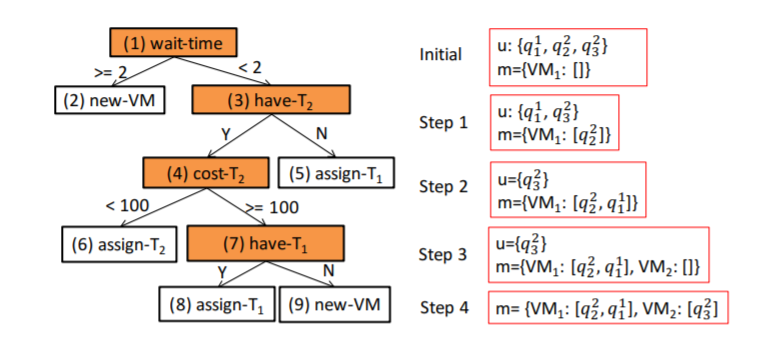
\includegraphics[width=1.0\textwidth]{decisiontree.PNG}
\caption{\label{fig:decision_tree}An example of a decision model}
\end{figure}

The right side of Figure~\ref{fig:decision_tree} shows how the decision tree is used to come up with the schedule for a workload \(Q = \{q^1_1, q^2_2, q^2_3\}\). Each query in \(T_1\) has a latency of two minutes and the goal is to execute it within three minutes. Instances of \(T_2\) have a latency of one minute and the goal is for each instance to be completed within one minute. For simplicity, we assume VMs of a single type and that queries are executed in isolation. 

Given this workload, the tree is parsed as follows. In the first node (1), we check the wait time, which is zero since all queries are unassigned, hence we proceed to node (3). The workload has queries of template \(T_2\) and therefore we proceed to node (4). Here we calculate the cost of placing an instance of \(T_2\). Let us assume the cost is is less than 100 (no penalty is incurred), which leads to node (6) which assigns an instance of \(T_2\) to the first VM. Since we have more queries in the workload we next re-parse the decision tree. In node (1) we check the wait time on the most recent VM which is now 1 minute (the runtime of queries of \(T_2\)) so we move to node (3). Since we have one more query of \(T_2\) unassigned, we move to (4). Now the cost of assigning a query of \(T_2\) is more than 100 since the new query would need to wait for \(q^2_1\) to complete (and thus incur a penalty). Hence, we move to node (7) and we check if there are any unassigned instances of \(T_1\). Since there are (\(q^1_1\)), we assign q11 to the last VM. We re-parse the tree in the same way and by following nodes \((1)\to(2)\), then again as \((1)\to(3)\to(4)\to(7)\to(9)\), so we assign the remaining query \(q^2_3\) onto a new VM. 

Each model represents a workload scheduling strategy. Given a batch of queries, the model in Figure 5 will place an instance of \(T_2\), then an instance of \(T_1\), and then create a new VM. This process will repeat itself until queries of \(T_1\) or \(T_2\) are depleted from the incoming batch. When all instances from one of the templates are assigned, single instances of the remaining template will be placed on new VMs until none remain.

\section{Random Forest}
Random forests \cite{liaw2002classification} or random decision forests are an ensemble learning method for classification, regression and other tasks, that operate by constructing a multitude of decision trees at training time and outputting the class that is the mode of the classes (classification) or mean prediction (regression) of the individual trees. Random decision forests correct for decision trees' habit of overfitting to their training set. We constructed Random forest on the data available and recorded the results which we will discuss in results chapter.

\section{Multiple VM-type systems}
In Multiple VM-type systems we should also decide which VM the system should initialise. To solve this we propose another feature named support-template-X. Further, If the cost of the query is very high for a VM of type j, then we can’t initialise such a VM. This feature tells the system whether the last recently used VM supports this query template.  Now, to choose the new VM, we introduce an approach in which we take the information regarding the queries we have and decide the VM that should be initialized. The model thus became a two decision supervised learning model. Whenever the first decision is an “Initialize VM”, a second decision will be taken by other classifier to choose the VM to be initialized. 

\begin{enumerate}
\item \textbf{Proportion-of-remaining-queries-supported-on-VM-type-Y:}\\
Proportion-of-remaining-queries-supported-on-VM-type-Y is the ratio between the number queries supported by the VM of type Y and the total number of queries left to be processed. For example, if there are four queries to be processed, with VM of type X supporting 2 and type Y supporting 3, then we extract the features Proportion-of-remaining-queries-supported-on-VM-type-X=0.5 and Proportion-of-remaining-queries-supported-on-VM-type-Y=0.75. Since each sample workload contains only a limited number of queries, keeping track of the exact number of instances of each query template would not scale to large workloads. Therefore, we track the proportion instead.
\item \textbf{Startup-Cost-of-type-Y:} The startup cost incurred by initializing a VM of type Y. Startup-Cost-of-type-Y is equal to the weight of the outgoing edge when we initialize a new VM. This allows our model to check the startup cost incurred by initializing a VM of a certain type and based on its value, decide which VM to assign.
\end {enumerate}